%%%%%%%%%%%%%%
%% Run LaTeX on this file several times to get Table of Contents,
%% cross-references, and citations.

%% If you have font problems, you may edit the w-bookps.sty file
%% to customize the font names to match those on your system.

%% w-bksamp.tex. Current Version: Feb 16, 2012
%%%%%%%%%%%%%%%%%%%%%%%%%%%%%%%%%%%%%%%%%%%%%%%%%%%%%%%%%%%%%%%%
%
%  Sample file for
%  Wiley Book Style, Design No.: SD 001B, 7x10
%  Wiley Book Style, Design No.: SD 004B, 6x9
%
%
%  Prepared by Amy Hendrickson, TeXnology Inc.
%  http://www.texnology.com
%%%%%%%%%%%%%%%%%%%%%%%%%%%%%%%%%%%%%%%%%%%%%%%%%%%%%%%%%%%%%%%%

%%%%%%%%%%%%%
% 7x10
%\documentclass{wileySev}

% 6x9

\documentclass{wileySix}

\documentclass{wileysix}


\usepackage{graphicx}
\usepackage{listings}

\usepackage{color}
 
\definecolor{codegreen}{rgb}{0,0.6,0}
\definecolor{codegray}{rgb}{0.5,0.5,0.5}
\definecolor{codepurple}{rgb}{0.58,0,0.82}
\definecolor{backcolour}{rgb}{0.95,0.95,0.92}
 
\lstdefinestyle{mystyle}{
    backgroundcolor=\color{backcolour},   
    commentstyle=\color{codegreen},
    keywordstyle=\color{magenta},
    numberstyle=\tiny\color{codegray},
    stringstyle=\color{codepurple},
    basicstyle=\footnotesize,
    breakatwhitespace=false,         
    breaklines=true,                 
    captionpos=b,                    
    keepspaces=true,                 
    numbers=left,                    
    numbersep=5pt,                  
    showspaces=false,                
    showstringspaces=false,
    showtabs=false,                  
    tabsize=2,
    language=sh
}
 
\lstset{style=mystyle}

%%%%%%%
%% for times math: However, this package disables bold math (!)
%% \mathbf{x} will still work, but you will not have bold math
%% in section heads or chapter titles. If you don't use math
%% in those environments, mathptmx might be a good choice.

% \usepackage{mathptmx}

% For PostScript text
\usepackage{w-bookps}

%%%%%%%%%%%%%%%%%%%%%%%%%%%%%%%%%%%%%%%%%%%%%%%%%%%%%%%%%%%%%%%%
%% Other packages you might want to use:

% for chapter bibliography made with BibTeX
% \usepackage{chapterbib}

% for multiple indices
% \usepackage{multind}

% for answers to problems
% \usepackage{answers}

%%%%%%%%%%%%%%%%%%%%%%%%%%%%%%
%% Change options here if you want:
%%
%% How many levels of section head would you like numbered?
%% 0= no section numbers, 1= section, 2= subsection, 3= subsubsection
%%==>>
\setcounter{secnumdepth}{3}

%% How many levels of section head would you like to appear in the
%% Table of Contents?
%% 0= chapter titles, 1= section titles, 2= subsection titles, 
%% 3= subsubsection titles.
%%==>>
\setcounter{tocdepth}{2}

%% Cropmarks? good for final page makeup
%% \docropmarks

%%%%%%%%%%%%%%%%%%%%%%%%%%%%%%
%
% DRAFT
%
% Uncomment to get double spacing between lines, current date and time
% printed at bottom of page.
% \draft
% (If you want to keep tables from becoming double spaced also uncomment
% this):
% \renewcommand{\arraystretch}{0.6}
%%%%%%%%%%%%%%%%%%%%%%%%%%%%%%

%%%%%%% Demo of section head containing sample macro:
%% To get a macro to expand correctly in a section head, with upper and
%% lower case math, put the definition and set the box 
%% before \begin{document}, so that when it appears in the 
%% table of contents it will also work:



%% use a box to expand the macro before we put it into the section head:

\newbox\sectsavebox
\setbox\sectsavebox=\hbox{\boldmath\VT{xyz}}

%%%%%%%%%%%%%%%%% End Demo


\begin{document}



\booktitle{PHP7: Buku Belajar Untuk Pemula Dan Awam Pemrograman }
\subtitle{Dalam 24 Jam}

\authors{Rolly M. Awangga\\
\affil{Informatics Research Center}




\offprintinfo{PHP7: Buku Belajar Untuk Pemula Dan Awam Pemrograman, First Edition}{Rolly M. Awangga}


%% Can use \\ if title, and edition are too wide, ie,
%% \offprintinfo{Survey Methodology,\\ Second Edition}{Robert M. Groves}

%%%%%%%%%%%%%%%%%%%%%%%%%%%%%%
%% 
\halftitlepage

\titlepage


\begin{copyrightpage}{2019}
%Survey Methodology / Robert M. Groves . . . [et al.].
%\       p. cm.---(Wiley series in survey methodology)
%\    ``Wiley-Interscience."
%\    Includes bibliographical references and index.
%\    ISBN 0-471-48348-6 (pbk.)
%\    1. Surveys---Methodology.  2. Social 
%\  sciences---Research---Statistical methods.  I. Groves, Robert M.  II. %
%Series.\\
%
%HA31.2.S873 2007
%001.4'33---dc22                                             2004044064
\end{copyrightpage}

\dedication{`Jika Kamu tidak dapat menahan lelahnya belajar, 
Maka kamu harus sanggup menahan perihnya Kebodohan.'
~Imam Syafi'i~}

\begin{contributors}
\name{Rolly Maulana Awangga,} Informatics Research Center., Politeknik Pos Indonesia, Bandung,
Indonesia



\end{contributors}

\contentsinbrief
\tableofcontents
\listoffigures
\listoftables
\lstlistoflistings


\begin{foreword}
Sepatah kata dari Kaprodi, Kabag Kemahasiswaan dan Mahasiswa
\end{foreword}

\begin{preface}
Buku ini diciptakan bagi yang awam dengan git sekalipun.

\prefaceauthor{R. M. Awangga}
\where{Bandung, Jawa Barat\\
Februari, 2019}
\end{preface}


\begin{acknowledgments}
Terima kasih atas semua masukan dari para mahasiswa agar bisa membuat buku ini 
lebih baik dan lebih mudah dimengerti.

Terima kasih ini juga ditujukan khusus untuk team IRC yang 
telah fokus untuk belajar dan memahami bagaimana buku ini mendampingi proses 
Intership.
\authorinitials{R. M. A.}
\end{acknowledgments}

\begin{acronyms}
\acro{ACGIH}{American Conference of Governmental Industrial Hygienists}
\acro{AEC}{Atomic Energy Commission}
\acro{OSHA}{Occupational Health and Safety Commission}
\acro{SAMA}{Scientific Apparatus Makers Association}
\end{acronyms}

\begin{glossary}
\term{git}Merupakan manajemen sumber kode yang dibuat oleh linus torvald.

\term{bash}Merupakan bahasa sistem operasi berbasiskan *NIX.

\term{linux}Sistem operasi berbasis sumber kode terbuka yang dibuat oleh Linus Torvald
\end{glossary}

\begin{symbols}
\term{A}Amplitude

\term{\hbox{\&}}Propositional logic symbol 

\term{a}Filter Coefficient

\bigskip

\term{\mathcal{B}}Number of Beats
\end{symbols}

\begin{introduction}

%% optional, but if you want to list author:

\introauthor{Rolly Maulana Awangga, S.T., M.T.}
{Informatics Research Center\\
Bandung, Jawa Barat, Indonesia}

Pada era disruptif  \index{disruptif}\index{disruptif!modern} 
saat ini. git merupakan sebuah kebutuhan dalam sebuah organisasi pengembangan perangkat lunak.
Buku ini diharapkan bisa menjadi penghantar para programmer, analis, IT Operation dan Project Manajer.
Dalam melakukan implementasi git pada diri dan organisasinya.

Rumusnya cuman sebagai contoh aja biar keren\cite{awangga2018sampeu}.

\begin{equation}
ABC {\cal DEF} \alpha\beta\Gamma\Delta\sum^{abc}_{def}
\end{equation}

\end{introduction}

%%%%%%%%%%%%%%%%%%Isi Buku_

\chapter{Judul Bagian Pertama}
<<<<<<< HEAD
\section{Pendahuluan}
	Situs web merupakan suatu layanan yang menyajikan informasi menggunakan konsep hyperlink, yang memudahkan pengguna dalam menelusuri atau mencari informasi dari internet untuk mendapatkan informasi, dengan cukup mengklik suatu link beupa teks atau gambar, maka dari teks atau gambar tersebut akan menampilkan informasi yang detail (rinci).
Informasi yang akan disajikan dalam halaman web menggunakan konsep multimedia, informasi dapat disajikan dengan menggunakan banyak media (teks, gambar, animasi, suara (audio), dan film). Dalam suatu halaman web, informasi akan disajikan dalam kombinasi dari media-media tersebut yang disajikan dalam suatu halaman.
	Situs web berupa kumpulan informasi yang disediakan secara perorangan, kelompok, atau organisasi. yang ditempatkan setidaknya pada sebuah server web yang dapat diakses melalui jaringan seperti Internet, ataupun jaringan wilayah lokal (LAN) melalui alamat Internet yang dikenali sebagai URL. Gabungan atas semua situs yang dapat diakses publik di Internet disebut pula sebagai World Wide Web atau lebih dikenal dengan singkatan WWW. Web merupakan hal yang sangat populer di lingkungan pengguna internet dalam mengakses dan mendapatkan informasi karena kemudahan yang diberikan kepada pengguna internet untuk melakukan penelusuran, penjelajahan dan pencarian informasi    
=======
\section{Pengenalan}
PHP adalah bahasa pemrograman script server-side yang didesain untuk pembuatan atau pengembangan web.
Dengan ini, PHP juga dapat digunakan sebagai bahasa pemrograman umum. PHP sendiri dikembangkan pada tahun 1995
oleh Rasmus Lerdorf, dan pada akhhirnya dikelola oleh The PHP Group. Situs resmi PHP beralamat http://www.php.net.
\par
PHP disebut bahasa pemrograman server side karena PHP diproses pada komputer server. 
Hal ini berbeda dibandingkan dengan bahasa pemrograman client-side seperti JavaScript yang diproses pada web browser (client).

>>>>>>> 295bf0df4a3cb6970f347bfe2e9d9ca4d639046d


\chapter{Judul Bagian Kedua}
\section{Perintah Navigasi}
Perintah navigasi direktori


\chapter{Dasar Penulisan PHP Sederhana}
\section{Aturan Dasar Penulisan Kode PHP}
Seperti bahasa pemograman yang lain, PHP juga memiliki aturan penulisan seperti case sensitifity (perbedaan antara huruf besar dan kecil), cara mengakhiri sebuah baris perintah, dan pengaruh penggunakan spasi dalam membuat kode program PHP. Berikut adalah aturan dasar penulisan kode PHP:
\subsection{Case Sensitivity (perbedaan huruf besar dan kecil) dalam PHP}
PHP tidak membedakan huruf besar dan kecil (case insensitive) untuk penamaan fungsi (function), nama class, maupun keyword bawaan PHP seperti echo, while, dan class. Ketiga baris berikut akan dianggap sama dalam PHP:
\begin{lstlisting}
<?php
Echo “Hello World”;
ECHO “Hello World”;
EchO “Hello World”;
?>
\end{lstlisting}
Akan tetapi, PHP membedakan huruf besar dan huruf kecil (case sensitive) untuk penamaan variabel, sehingga akan dianggap sebagai variabel yang berbeda. Sering kali error terjadi dikarenakan salah menuliskan nama variabel, yang seharusnya menggunakan huruf kecil, ditulis dengan huruf besar.
\begin{lstlisting}
<?php
$luqman="Luqman";
echo $Luqman; // Notice: Undefined variable: Luqman
?>
\end{lstlisting}
Untuk mengatasi perbedaan ini, disarankan menggunakan huruf kecil untuk seluruh kode PHP, termasuk variabel, fungsi maupun class. Jika membutuhkan nama variabel yang terdiri dari 2 kata, karakter spasi bisa digantikan dengan underscore.
\subsection{Karakter Spasi dan Tab dalam PHP}
Dalam PHP, karakter seperti spasi dan tab diabaikan di dalam eksekusi program PHP. Anda boleh mencoba sebuah statement menjadi beberapa baris, atau menyatukan beberapa statement dalam sebuah baris yang lumayan panjang. Seperti contoh berikut:
\begin{lstlisting}
<?php
echo "Saya belajar"; echo "Saya mengerti"; $nama="Men";
?>
\end{lstlisting}
Baris statement itu sama dengan
 \begin{lstlisting}
<?php
     echo "Saya belajar";
     echo "Saya mengerti";
     $nama = "Men";
?>
\end{lstlisting}
Walaupun contoh yang pertama lebih menghemat baris, namun lebih disarankan untuk contoh kedua, karena kita mengusahakan agar setiap statement berada dalam satu baris saja, dan menambahkan beberapa spasi di awal untuk memudahkan membaca kode program.
\par
Keuntungan penghematan baris dan beberapa byte dari sebuah file PHP tidak akan sebanding dengan mencoba memahami kode program yang dibuat dalam beberapa hari kedepan. Menambahkan sebagian komentar pada bagian kode yang lebih rumit sebagai penjelasan juga sangat disarankan.
\section{Embedded Script dan Non Embedded}
\subsection{Embedded Script}
  \item Berikut merupakan contoh dokumen HTML yang akan dihasilkan dengan menggunakan program/script PHP dalam embedded script
    Ditampilkan dibawah ini  :
    \lstinputlisting[firstline=1, lastline=12]{src/embedded_script.php}
Script diatas menunjukkan contoh script PHP sederhana yang disebut dengan script embedded yang di sisipkan diantara tag-tag HTML. Script tersebut digunakan apabila isi dari suatu dokumen HTML diinginkan dari hasil eksekusi suatu script PHP. jika dilihat dari source-nya dengan menggunakan view source pada web browser maka tampilannya akan berupa seperti berikut
    \lstinputlisting[firstline=14, lastline=22]{src/embedded_script.php}
Source dokumen HTML yang tampil berupa dokumen HTML yang tidak lagi dari script PHP yang berisi script PHP karena semua menjadi tag HTML, karena pada saat dieksekusi maka bukan scriptnya yang dikirim tetapi eksekusi dari script tersebut yang dikirim 
\subsection{Non Embedded}
   \item Script PHP dibawah ini merupakan script murni dari pembuatan program dengan menggunakan PHP, tag dokumen HTML yang dihasilkan untuk membuat dokumen merupakan bagian dari script PHP. di tampilkan dibawah ini:
  \lstinputlisting[firstline=24, lastline=35]{src/embedded_script.php}
dan dibawah ini merupakan source dokumen HTML dari tampilan kode diatas  
  \lstinputlisting[firstline=38, lastline=40]{src/embedded_script.php}
Jika diperhatikan dokumen HTML tersebut tidak beraturan ditampilkan. Hal tersebut tidak menjadi masalah, yang penting adalah browser web dapat menampilkannya, karena dokumen tag HTML ini murni dihasilkan dari script PHP. 
\section{Variabel dan Tipe Data}
\subsection{Variabel}
Variabel adalah tempat penympanan data, variabel memiliki nama. dalam pemograman variabel merupakan tempat penyimpanan data didalam memori komputer. Didalam PHP nama variabel diawali dengan karakter dollar diikuti dengan huruf sebagai karakter pertama setelah dollar. kemudian kombinasi karakter dan angka. Tidak boleh ada spasi dan tanda baca dalam penamaannya. kecuali karakter (garis bawah, under score).berikut merupakan penulisan variabel yang benar:
\lstinputlisting[firstline=31, lastline=34]{src/tag_awal_akhir.php}
\subsection{Tipe Data}
Data yang diolah oleh suatu program memiliki berbagai jenis ada data yang menunjukkan jumlah dan menunjukkan nilai benar dan salah, atau tulisan. Jenis tipe data dalam PHP secara mendasar dibedakan menjadi 3 macam yang disebut sebagai tipe data primitif. Tipe data primitif yang diolah oleh PHP:
\begin{enumerate}
\item Numerik
\item String
\item Boolean
\end{enumerate}
Tipe data numerik dibedakan menjadi tipe data integer dan flooting point. Selain itu tipe data yang lain adalah tipe data compound, terdiri atas:
\begin{enumerate}
\item tipe data array
\item tipe data objek 
\end{enumerate}
\subsection{Tipe Data Integer}
 tipe data integer adalah tipe data yang terdiri dari angka bulat (tidak mengandung nilai pecahan atau nilai desimal). Nilai ini bisa berbentuk angka positif maupun negatif, contohnya 1, 2, 6, -44, 20000, atau 128730123. Tipe data integer dapat dituliskan dengan notasi sebagai berikut
\begin{enumerate}
\item Notasi Desimal adalah susunan bilangan yang mempunyai basis sepuluh. 
Koefisien bilangan desimal terdiri dari 0,1,2,3,4,5,6,7,8,9.
Notasi bilangan desimal dituliskan: (n)10
\item Notasi Oktal adalah susunan bilangan yang mempunyai basis delapan. 
Koefisien bilangan oktal terdiri dari 0,1,2,3,4,5,6,7.
Notasi bilangan oktal dituliskan : (n)8
\item Biner adalah susunan bilangan yang mempunyai basis dua. 
Basis dua di sini adalah nilai koefisien yaitu 0 dan 1.
Notasi bilangan biner dituliskan : (n)2
\item Notasi Heksadesimal adalah susunan bilangan yang mempunyai basis enam belas. 
Koefisien bilangan heksadesimal terdiri dari 0,1,2,3,4,5,6,7,8,9,A,B,C,D,F.

Catatan: A bernilai 10, B bernilai 11, ... , F bernilai 15.
Notasi bilangan hekasdesimal dituliskan : (n)16

\begin{figure}[!htbp]
 \centering
 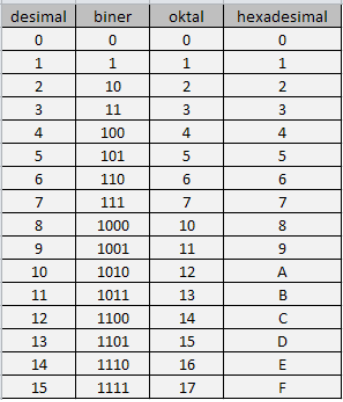
\includegraphics[width=.50\textwidth]{figures/sistem_bilangan.png}
 \caption{Sistem Bilangan}\label{fig:inputchapter}
\end{figure}

\end{enumerate}

\subsection{Tipe Data Floting Point}
Tipe data float (disebut juga tipe data floating point, atau real number) adalah tipe data angka yang memiliki bagian desimal di akhir angka, atau memiliki floating point (floating point adalah istilah dalam bahasa inggris untuk menyebut tanda “titik” yang menandakan bilangan desimal). Contoh angka float adalah seperti: 0,9 atau 3,14. Tipe data float cocok digunakan untuk variabel yang akan berisi angka pecahan, seperti nilai IPK, hasil pembagian, atau hasil komputasi numerik yang angkanya tidak bisa ditampung oleh data integer.
\subsection{Tipe Data String}
Tipe data String adalah tipe data untuk teks yang merupakan gabungan huruf, angka, whitespace (spasi), dan berbagai karakter. Fungsi ini digunakan untuk membuat identifier String/teks. Data string ditulis dengan mengapit data string tersebut dengan tanda petik tunggal atau tanda petik ganda. Tanda petik tunggal umumnya digunakan sebagai konstanta string.
\subsection{Tipe Data Boolean}
Tipe data boolean sebenarnya sangat sederhana. Tipe data ini hanya bisa diisi dengan salah satu dari 2 nilai: TRUE atau FALSE. Tipe data boolean banyak dipakai dalam percabangan kode program, atau untuk memutuskan apa yang harus dijalankan pada sebuah kondisi if else.
\subsection{Tipe Data Objek}
Tipe data dari objek merupakan tipe data baru, merupakan pengembangan PHP untuk mendukung program berorientasi objek. Tipe data objek adalah tipe data yang didalamnya mempunyai data dan method. data yang dipunyai oleh suatu objek populer dengan nama atribut dan method suatu objek umumnya berupa suatu fungsi. 

Data objek didefinisikan dengan membuat definisi kelas terlebih dahulu. Suatu variabel yang bertipe objek diinisialisasi (dideklarasi) dengan menggunakan perintah new kemudian nama objek (berupa nama kelas objek) berikut contohnya:
\lstinputlisting[firstline=1, lastline=17]{src/tipeDataObjek.php}


\section{Operator PHP}
Pada PHP, terdapat banyak operator  beberapa yang sering digunakan.
\subsection{Operator Perbandigan}
Seperti namanya, operator perbandingan digunakan untuk membandingkan beberapa buah nilai pada PHP dan hasilnya berupa booelan true yang berarti benar atau false yang berarti salah.
Contoh:
\begin{lstlisting}
<?php
if ($_POST['password'] == 'admin')
{
	echo 'Login sukses';
}
\end{lstlisting}

\subsection{ Operator PHP Increment dan Decrement}
Operator ini digunakan untuk menambahkan atau mengurangi nilai sebanyak 1 pada suatu variabel. 
\subsection{Perbedaan Pre Increment dan Post Increment}
Pada pre increment, nilai variabel akan ditambahkan 1 baru kemudian siap digunakan, sebaliknya, untuk  post increment, gunakan dulu nilai variabel kemudian baru ditambahkan dengan 1.
Contoh 1:
\begin{lstlisting}
<?php
$nomor = 1;
while($nomor <= 5) {
	echo $nomor++;
}
\end{lstlisting}
Contoh diatas akan menghasilkan angka 12345.

Contoh 2:
\begin{lstlisting}
<?php
$nomor = 1;
while($nomor <= 5) {
	echo ++$nomor;
}
\end{lstlisting}
Contoh diatas akan menghasilkan 23456.
Lihat, perbedaanya terdapat pada ++ sebelum dan sesudah $nomor. 

\subsection{Operator Assignment PHP}
Sesuai namanya Assignment operator ini digunakan untuk memberikan nilai pada suatu variabel. Operator dasarnya adalah tanda sama dengan ( = ). Dalam praktiknya, operator ini sering digunakan ketika menjumlahkan nilai pada suatu perulangan, seperti ketika menjumlahkan data hasil query database.
Contoh:
\begin{lstlisting}
<?php
$sql 	= 'SELECT * FROM sales';
$query 	= mysqli_query($sql);
$total	= 0;
while($row = mysqli_fetch_array($query))
{
	$total += $row['jml_bayar'];
}
\end{lstlisting}

\section{Lingkup Variabel}
Variabel Scope (atau ruang lingkup variabel) adalah jangkauan kode program dimana perintah program masih bisa mengakses sebuah variabel. Variabel menunjukkan keberlakuan dan dikenalinya suatu variabel didalam script. Suatu variabel yang didefinisikan didalam sebuah fungsi maka variabel tersebut hanya akan dikenali dan digunakan hanya dalam fungsi tersebut variabel ini dikenal sebagai variabel lokal. karena hanya dikenal pada fungsi tempat variabel tersebut dinyatakan dan digunakan.

Jika kita mendefenisikan sebuah variabel pada satu file PHP, maka variabel tersebut dapat diakses oleh seluruh kode program pada halaman yang sama. Namun jika variabel tersebut di defenisikan di dalam sebuah fungsi, variabel itu belum tentu bisa diakses dari luar fungsi tersebut. Hal inilah yang dimaksud dengan Variabel Scope. Variabel akan disebut global apabila variabel tersebut dapat dikenali dan digunakan oleh seluruh bagian script tersebut

Variabel yang didefenisikan di dalam sebuah fungsi, secara default tidak dapat diakses oleh kode program di luar fungsi tersebut. Dan begitu juga sebaliknya, variabel yang didefenisikan di luar fungsi, tidak bisa diakses dari dalam fungsi. Berikut jenis variabel berdasarkan lingkupnya:

\subsection{Variabel Global}
\subsection{Variabel Lokal}
\subsection{Variabel Statik}




\bibliographystyle{IEEEtran} 
%\def\bibfont{\normalsize}
\bibliography{references}


%%%%%%%%%%%%%%%
%%  The default LaTeX Index
%%  Don't need to add any commands before \begin{document}
\printindex


%%%% Making an index
%% 
%% 1. Make index entries, don't leave any spaces so that they
%% will be sorted correctly.
%% 
%% \index{term}
%% \index{term!subterm}
%% \index{term!subterm!subsubterm}
%% 
%% 2. Run LaTeX several times to produce <filename>.idx
%% 
%% 3. On command line, type  makeindx <filename> which
%% will produce <filename>.ind 
%% 
%% 4. Type \printindex to make the index appear in your book.
%% 
%% 5. If you would like to edit <filename>.ind 
%% you may do so. See docs.pdf for more information.
%% 
%%%%%%%%%%%%%%%%%%%%%%%%%%%%%%

%%%%%%%%%%%%%% Making Multiple Indices %%%%%%%%%%%%%%%%
%% 1. 
%% \usepackage{multind}
%% \makeindex{book}
%% \makeindex{authors}
%% \begin{document}
%% 
%% 2.
%% % add index terms to your book, ie,
%% \index{book}{A term to go to the topic index}
%% \index{authors}{Put this author in the author index}
%% 
%% \index{book}{Cows}
%% \index{book}{Cows!Jersey}
%% \index{book}{Cows!Jersey!Brown}
%% 
%% \index{author}{Douglas Adams}
%% \index{author}{Boethius}
%% \index{author}{Mark Twain}
%% 
%% 3. On command line type 
%% makeindex topic 
%% makeindex authors
%% 
%% 4.
%% this is a Wiley command to make the indices print:
%% \multiprintindex{book}{Topic index}
%% \multiprintindex{authors}{Author index}

\end{document}

